\documentclass[twoside]{book}

% Packages required by doxygen
\usepackage{fixltx2e}
\usepackage{calc}
\usepackage{doxygen}
\usepackage[export]{adjustbox} % also loads graphicx
\usepackage{graphicx}
\usepackage[utf8]{inputenc}
\usepackage{makeidx}
\usepackage{multicol}
\usepackage{multirow}
\PassOptionsToPackage{warn}{textcomp}
\usepackage{textcomp}
\usepackage[nointegrals]{wasysym}
\usepackage[table]{xcolor}

% Font selection
\usepackage[T1]{fontenc}
\usepackage[scaled=.90]{helvet}
\usepackage{courier}
\usepackage{amssymb}
\usepackage{sectsty}
\renewcommand{\familydefault}{\sfdefault}
\allsectionsfont{%
  \fontseries{bc}\selectfont%
  \color{darkgray}%
}
\renewcommand{\DoxyLabelFont}{%
  \fontseries{bc}\selectfont%
  \color{darkgray}%
}
\newcommand{\+}{\discretionary{\mbox{\scriptsize$\hookleftarrow$}}{}{}}

% Page & text layout
\usepackage{geometry}
\geometry{%
  a4paper,%
  top=2.5cm,%
  bottom=2.5cm,%
  left=2.5cm,%
  right=2.5cm%
}
\tolerance=750
\hfuzz=15pt
\hbadness=750
\setlength{\emergencystretch}{15pt}
\setlength{\parindent}{0cm}
\setlength{\parskip}{3ex plus 2ex minus 2ex}
\makeatletter
\renewcommand{\paragraph}{%
  \@startsection{paragraph}{4}{0ex}{-1.0ex}{1.0ex}{%
    \normalfont\normalsize\bfseries\SS@parafont%
  }%
}
\renewcommand{\subparagraph}{%
  \@startsection{subparagraph}{5}{0ex}{-1.0ex}{1.0ex}{%
    \normalfont\normalsize\bfseries\SS@subparafont%
  }%
}
\makeatother

% Headers & footers
\usepackage{fancyhdr}
\pagestyle{fancyplain}
\fancyhead[LE]{\fancyplain{}{\bfseries\thepage}}
\fancyhead[CE]{\fancyplain{}{}}
\fancyhead[RE]{\fancyplain{}{\bfseries\leftmark}}
\fancyhead[LO]{\fancyplain{}{\bfseries\rightmark}}
\fancyhead[CO]{\fancyplain{}{}}
\fancyhead[RO]{\fancyplain{}{\bfseries\thepage}}
\fancyfoot[LE]{\fancyplain{}{}}
\fancyfoot[CE]{\fancyplain{}{}}
\fancyfoot[RE]{\fancyplain{}{\bfseries\scriptsize Generated by Doxygen }}
\fancyfoot[LO]{\fancyplain{}{\bfseries\scriptsize Generated by Doxygen }}
\fancyfoot[CO]{\fancyplain{}{}}
\fancyfoot[RO]{\fancyplain{}{}}
\renewcommand{\footrulewidth}{0.4pt}
\renewcommand{\chaptermark}[1]{%
  \markboth{#1}{}%
}
\renewcommand{\sectionmark}[1]{%
  \markright{\thesection\ #1}%
}

% Indices & bibliography
\usepackage{natbib}
\usepackage[titles]{tocloft}
\setcounter{tocdepth}{3}
\setcounter{secnumdepth}{5}
\makeindex

% Hyperlinks (required, but should be loaded last)
\usepackage{ifpdf}
\ifpdf
  \usepackage[pdftex,pagebackref=true]{hyperref}
\else
  \usepackage[ps2pdf,pagebackref=true]{hyperref}
\fi
\hypersetup{%
  colorlinks=true,%
  linkcolor=blue,%
  citecolor=blue,%
  unicode%
}

% Custom commands
\newcommand{\clearemptydoublepage}{%
  \newpage{\pagestyle{empty}\cleardoublepage}%
}

\usepackage{caption}
\captionsetup{labelsep=space,justification=centering,font={bf},singlelinecheck=off,skip=4pt,position=top}

%===== C O N T E N T S =====

\begin{document}

% Titlepage & ToC
\hypersetup{pageanchor=false,
             bookmarksnumbered=true,
             pdfencoding=unicode
            }
\pagenumbering{roman}
\begin{titlepage}
\vspace*{7cm}
\begin{center}%
{\Large Image C \\[1ex]\large 1.\+0 }\\
\vspace*{1cm}
{\large Generated by Doxygen 1.8.11}\\
\end{center}
\end{titlepage}
\clearemptydoublepage
\tableofcontents
\clearemptydoublepage
\pagenumbering{arabic}
\hypersetup{pageanchor=true}

%--- Begin generated contents ---
\chapter{Hierarchical Index}
\section{Class Hierarchy}
This inheritance list is sorted roughly, but not completely, alphabetically\+:\begin{DoxyCompactList}
\item \contentsline{section}{Condition}{\pageref{class_condition}}{}
\begin{DoxyCompactList}
\item \contentsline{section}{Est\+Petite}{\pageref{class_est_petite}}{}
\item \contentsline{section}{Est\+Un}{\pageref{class_est_un}}{}
\item \contentsline{section}{Et}{\pageref{class_et}}{}
\item \contentsline{section}{Non}{\pageref{class_non}}{}
\end{DoxyCompactList}
\item Figure\begin{DoxyCompactList}
\item \contentsline{section}{Cercle}{\pageref{class_cercle}}{}
\item \contentsline{section}{Image}{\pageref{class_image}}{}
\item \contentsline{section}{Line}{\pageref{class_line}}{}
\item \contentsline{section}{Rectangle}{\pageref{class_rectangle}}{}
\item \contentsline{section}{Triangle}{\pageref{class_triangle}}{}
\end{DoxyCompactList}
\item \contentsline{section}{Filtrage}{\pageref{class_filtrage}}{}
\item \contentsline{section}{Matrice2D}{\pageref{class_matrice2_d}}{}
\item \contentsline{section}{Point}{\pageref{class_point}}{}
\item \contentsline{section}{Shape}{\pageref{class_shape}}{}
\end{DoxyCompactList}

\chapter{Class Index}
\section{Class List}
Here are the classes, structs, unions and interfaces with brief descriptions\+:\begin{DoxyCompactList}
\item\contentsline{section}{\hyperlink{class_cercle}{Cercle} }{\pageref{class_cercle}}{}
\item\contentsline{section}{\hyperlink{class_condition}{Condition} }{\pageref{class_condition}}{}
\item\contentsline{section}{\hyperlink{class_est_petite}{Est\+Petite} }{\pageref{class_est_petite}}{}
\item\contentsline{section}{\hyperlink{class_est_un}{Est\+Un} }{\pageref{class_est_un}}{}
\item\contentsline{section}{\hyperlink{class_et}{Et} }{\pageref{class_et}}{}
\item\contentsline{section}{\hyperlink{class_filtrage}{Filtrage} }{\pageref{class_filtrage}}{}
\item\contentsline{section}{\hyperlink{class_image}{Image} }{\pageref{class_image}}{}
\item\contentsline{section}{\hyperlink{class_line}{Line} }{\pageref{class_line}}{}
\item\contentsline{section}{\hyperlink{class_matrice2_d}{Matrice2D} }{\pageref{class_matrice2_d}}{}
\item\contentsline{section}{\hyperlink{class_non}{Non} }{\pageref{class_non}}{}
\item\contentsline{section}{\hyperlink{class_point}{Point} }{\pageref{class_point}}{}
\item\contentsline{section}{\hyperlink{class_rectangle}{Rectangle} }{\pageref{class_rectangle}}{}
\item\contentsline{section}{\hyperlink{class_shape}{Shape} }{\pageref{class_shape}}{}
\item\contentsline{section}{\hyperlink{class_triangle}{Triangle} }{\pageref{class_triangle}}{}
\end{DoxyCompactList}

\chapter{File Index}
\section{File List}
Here is a list of all documented files with brief descriptions\+:\begin{DoxyCompactList}
\item\contentsline{section}{archive/{\bfseries cercle.\+hpp} }{\pageref{cercle_8hpp}}{}
\item\contentsline{section}{archive/{\bfseries condition.\+h} }{\pageref{condition_8h}}{}
\item\contentsline{section}{archive/{\bfseries est\+Petite.\+h} }{\pageref{est_petite_8h}}{}
\item\contentsline{section}{archive/{\bfseries est\+Un.\+h} }{\pageref{est_un_8h}}{}
\item\contentsline{section}{archive/{\bfseries et.\+h} }{\pageref{et_8h}}{}
\item\contentsline{section}{archive/{\bfseries filtrage.\+h} }{\pageref{filtrage_8h}}{}
\item\contentsline{section}{archive/{\bfseries image.\+hpp} }{\pageref{image_8hpp}}{}
\item\contentsline{section}{archive/{\bfseries non.\+h} }{\pageref{non_8h}}{}
\item\contentsline{section}{archive/{\bfseries rectangle.\+hpp} }{\pageref{rectangle_8hpp}}{}
\item\contentsline{section}{archive/{\bfseries triangle.\+hpp} }{\pageref{triangle_8hpp}}{}
\item\contentsline{section}{include/{\bfseries Line.\+hpp} }{\pageref{_line_8hpp}}{}
\item\contentsline{section}{include/{\bfseries Matrice2\+D.\+hpp} }{\pageref{_matrice2_d_8hpp}}{}
\item\contentsline{section}{include/{\bfseries Point.\+hpp} }{\pageref{_point_8hpp}}{}
\item\contentsline{section}{include/{\bfseries Shape.\+hpp} }{\pageref{_shape_8hpp}}{}
\item\contentsline{section}{src/\hyperlink{_line_8cpp}{Line.\+cpp} \\*Implementation d\textquotesingle{}une ligne }{\pageref{_line_8cpp}}{}
\end{DoxyCompactList}

\chapter{Class Documentation}
\hypertarget{class_cercle}{}\section{Cercle Class Reference}
\label{class_cercle}\index{Cercle@{Cercle}}


Inheritance diagram for Cercle\+:
\nopagebreak
\begin{figure}[H]
\begin{center}
\leavevmode
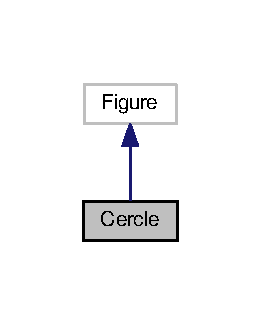
\includegraphics[width=125pt]{class_cercle__inherit__graph}
\end{center}
\end{figure}


Collaboration diagram for Cercle\+:
\nopagebreak
\begin{figure}[H]
\begin{center}
\leavevmode
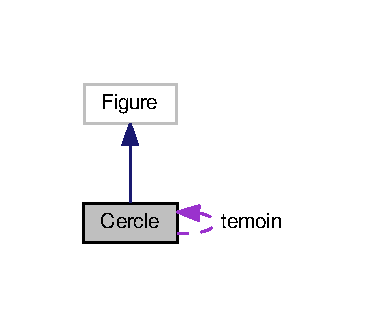
\includegraphics[width=176pt]{class_cercle__coll__graph}
\end{center}
\end{figure}
\subsection*{Public Member Functions}
\begin{DoxyCompactItemize}
\item 
{\bfseries Cercle} (const \hyperlink{class_point}{Point} \&centre=\hyperlink{class_point}{Point}(0, 0), int rayon=0)\hypertarget{class_cercle_a86f7651e775f5c93e862bfa7972bf56f}{}\label{class_cercle_a86f7651e775f5c93e862bfa7972bf56f}

\item 
\hyperlink{class_point}{Point} {\bfseries get\+Centre} () const \hypertarget{class_cercle_ad107d1ad2b6e5e892fcb70d82f36ebdb}{}\label{class_cercle_ad107d1ad2b6e5e892fcb70d82f36ebdb}

\item 
int {\bfseries get\+Rayon} () const \hypertarget{class_cercle_a9cc2d88b4d0661247ef43923738fd99c}{}\label{class_cercle_a9cc2d88b4d0661247ef43923738fd99c}

\item 
virtual Figure $\ast$ \hyperlink{class_cercle_ac575daf278545708579a610755c2e05b}{copy} () const 
\item 
virtual list$<$ \hyperlink{class_point}{Point} $\ast$ $>$ {\bfseries get\+Points} () const \hypertarget{class_cercle_aa03de04f35262772b7e47bb1aedd6adb}{}\label{class_cercle_aa03de04f35262772b7e47bb1aedd6adb}

\item 
virtual void \hyperlink{class_cercle_a32d66b80b939c817e5ac6719f6416410}{deplacer} (const \hyperlink{class_point}{Point} \&trans)
\item 
virtual void \hyperlink{class_cercle_a329f70e491ef800167074fa0732c550d}{dessiner} (ostream \&os=cout) const 
\item 
virtual double {\bfseries surface} () const \hypertarget{class_cercle_a134ec3bb605c3fde159b0b0ae37c7330}{}\label{class_cercle_a134ec3bb605c3fde159b0b0ae37c7330}

\item 
virtual double {\bfseries perimetre} () const \hypertarget{class_cercle_ac3cb41e2afe36ae5c25e544039267b39}{}\label{class_cercle_ac3cb41e2afe36ae5c25e544039267b39}

\item 
virtual double {\bfseries distance\+\_\+origine} (const \hyperlink{class_point}{Point} \&p) const \hypertarget{class_cercle_a7ee40532a986a25b6a36f3e0462ebbc6}{}\label{class_cercle_a7ee40532a986a25b6a36f3e0462ebbc6}

\item 
virtual void {\bfseries afficher} (ostream \&os=cout) const \hypertarget{class_cercle_a5ff7c5a68ed50b44fe7ec402b7ed58fb}{}\label{class_cercle_a5ff7c5a68ed50b44fe7ec402b7ed58fb}

\end{DoxyCompactItemize}
\subsection*{Static Public Attributes}
\begin{DoxyCompactItemize}
\item 
static \hyperlink{class_cercle}{Cercle} \hyperlink{class_cercle_a804c15697f2286eca717d04c6450e12e}{temoin} = \hyperlink{class_cercle}{Cercle}(\hyperlink{class_point}{Point}(0,0), 0)
\end{DoxyCompactItemize}


\subsection{Member Function Documentation}
\index{Cercle@{Cercle}!copy@{copy}}
\index{copy@{copy}!Cercle@{Cercle}}
\subsubsection[{\texorpdfstring{copy() const }{copy() const }}]{\setlength{\rightskip}{0pt plus 5cm}Figure $\ast$ Cercle\+::copy (
\begin{DoxyParamCaption}
{}
\end{DoxyParamCaption}
) const\hspace{0.3cm}{\ttfamily [virtual]}}\hypertarget{class_cercle_ac575daf278545708579a610755c2e05b}{}\label{class_cercle_ac575daf278545708579a610755c2e05b}
Fonction virtuelle de copie \index{Cercle@{Cercle}!deplacer@{deplacer}}
\index{deplacer@{deplacer}!Cercle@{Cercle}}
\subsubsection[{\texorpdfstring{deplacer(const Point \&trans)}{deplacer(const Point &trans)}}]{\setlength{\rightskip}{0pt plus 5cm}void Cercle\+::deplacer (
\begin{DoxyParamCaption}
\item[{const {\bf Point} \&}]{p}
\end{DoxyParamCaption}
)\hspace{0.3cm}{\ttfamily [virtual]}}\hypertarget{class_cercle_a32d66b80b939c817e5ac6719f6416410}{}\label{class_cercle_a32d66b80b939c817e5ac6719f6416410}
D�placement-\/translation de valeur le point p \index{Cercle@{Cercle}!dessiner@{dessiner}}
\index{dessiner@{dessiner}!Cercle@{Cercle}}
\subsubsection[{\texorpdfstring{dessiner(ostream \&os=cout) const }{dessiner(ostream &os=cout) const }}]{\setlength{\rightskip}{0pt plus 5cm}void Cercle\+::dessiner (
\begin{DoxyParamCaption}
\item[{ostream \&}]{os = {\ttfamily cout}}
\end{DoxyParamCaption}
) const\hspace{0.3cm}{\ttfamily [virtual]}}\hypertarget{class_cercle_a329f70e491ef800167074fa0732c550d}{}\label{class_cercle_a329f70e491ef800167074fa0732c550d}
Le dessin se limite � un affichage 

\subsection{Member Data Documentation}
\index{Cercle@{Cercle}!temoin@{temoin}}
\index{temoin@{temoin}!Cercle@{Cercle}}
\subsubsection[{\texorpdfstring{temoin}{temoin}}]{\setlength{\rightskip}{0pt plus 5cm}{\bf Cercle} Cercle\+::temoin = {\bf Cercle}({\bf Point}(0,0), 0)\hspace{0.3cm}{\ttfamily [static]}}\hypertarget{class_cercle_a804c15697f2286eca717d04c6450e12e}{}\label{class_cercle_a804c15697f2286eca717d04c6450e12e}
auteurs \+: Michel Landschoot mail \+: \href{mailto:direction@landsnet.com}{\tt direction@landsnet.\+com} date de cr�ation \+: 2013-\/12-\/21 description \+: impl�m�ntation d\textquotesingle{}une classe d�crivant un cercle dans une hi�rachie de figures Le cercle t�moin est une variable de classe 

The documentation for this class was generated from the following files\+:\begin{DoxyCompactItemize}
\item 
archive/cercle.\+hpp\item 
archive/cercle.\+cpp\end{DoxyCompactItemize}

\hypertarget{class_condition}{}\section{Condition Class Reference}
\label{class_condition}\index{Condition@{Condition}}


{\ttfamily \#include $<$condition.\+h$>$}



Inheritance diagram for Condition\+:
\nopagebreak
\begin{figure}[H]
\begin{center}
\leavevmode
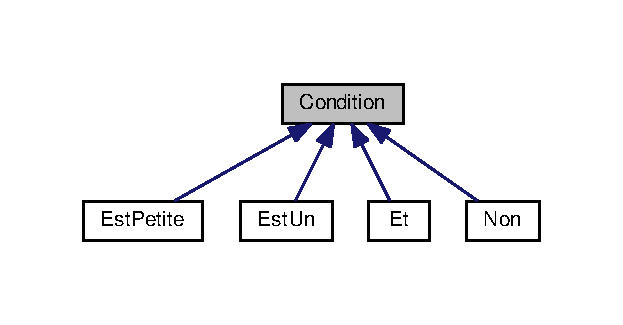
\includegraphics[width=299pt]{class_condition__inherit__graph}
\end{center}
\end{figure}
\subsection*{Public Member Functions}
\begin{DoxyCompactItemize}
\item 
virtual bool {\bfseries verif} (const Figure $\ast$f) const =0\hypertarget{class_condition_a3d02f40ff7b7cf7610e1a5ab8030a009}{}\label{class_condition_a3d02f40ff7b7cf7610e1a5ab8030a009}

\item 
virtual string {\bfseries to\+String} () const =0\hypertarget{class_condition_af5d835f98dbe6f45916d597008606be4}{}\label{class_condition_af5d835f98dbe6f45916d597008606be4}

\end{DoxyCompactItemize}


\subsection{Detailed Description}
auteurs \+: Michel Landschoot mail \+: \href{mailto:direction@landsnet.com}{\tt direction@landsnet.\+com} date de cr�ation \+: 2013-\/12-\/21 description \+: classe abstraite de base d\textquotesingle{}une hi�rarchie de conditions

La classe \hyperlink{class_condition}{Condition} devrait proposer une fonction de copie virtuelle � l\textquotesingle{}instar de la classe Figure 

The documentation for this class was generated from the following file\+:\begin{DoxyCompactItemize}
\item 
archive/condition.\+h\end{DoxyCompactItemize}

\hypertarget{class_est_petite}{}\section{Est\+Petite Class Reference}
\label{class_est_petite}\index{Est\+Petite@{Est\+Petite}}


Inheritance diagram for Est\+Petite\+:
\nopagebreak
\begin{figure}[H]
\begin{center}
\leavevmode
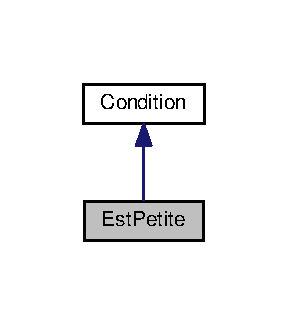
\includegraphics[width=138pt]{class_est_petite__inherit__graph}
\end{center}
\end{figure}


Collaboration diagram for Est\+Petite\+:
\nopagebreak
\begin{figure}[H]
\begin{center}
\leavevmode
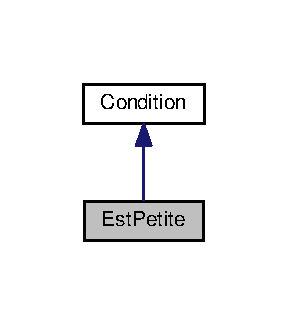
\includegraphics[width=138pt]{class_est_petite__coll__graph}
\end{center}
\end{figure}
\subsection*{Public Member Functions}
\begin{DoxyCompactItemize}
\item 
{\bfseries Est\+Petite} (double seuil)\hypertarget{class_est_petite_af8f816b95d9a14dc7629fa16de267f00}{}\label{class_est_petite_af8f816b95d9a14dc7629fa16de267f00}

\item 
double {\bfseries get\+Seuil} () const \hypertarget{class_est_petite_ad61c2808fedec928fc3b306a62e648ee}{}\label{class_est_petite_ad61c2808fedec928fc3b306a62e648ee}

\item 
virtual string {\bfseries to\+String} () const \hypertarget{class_est_petite_adb7ca26ffd55246f9f3054c711dfdc14}{}\label{class_est_petite_adb7ca26ffd55246f9f3054c711dfdc14}

\item 
virtual bool {\bfseries verif} (const Figure $\ast$f) const \hypertarget{class_est_petite_a81a65daa468125807a527178307f138b}{}\label{class_est_petite_a81a65daa468125807a527178307f138b}

\end{DoxyCompactItemize}


The documentation for this class was generated from the following file\+:\begin{DoxyCompactItemize}
\item 
archive/est\+Petite.\+h\end{DoxyCompactItemize}

\hypertarget{class_est_un}{}\section{Est\+Un Class Reference}
\label{class_est_un}\index{Est\+Un@{Est\+Un}}


{\ttfamily \#include $<$est\+Un.\+h$>$}



Inheritance diagram for Est\+Un\+:
\nopagebreak
\begin{figure}[H]
\begin{center}
\leavevmode
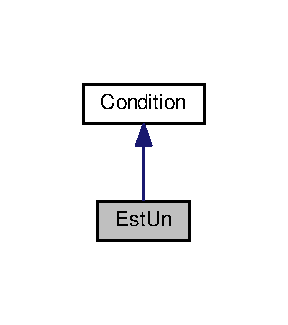
\includegraphics[width=138pt]{class_est_un__inherit__graph}
\end{center}
\end{figure}


Collaboration diagram for Est\+Un\+:
\nopagebreak
\begin{figure}[H]
\begin{center}
\leavevmode
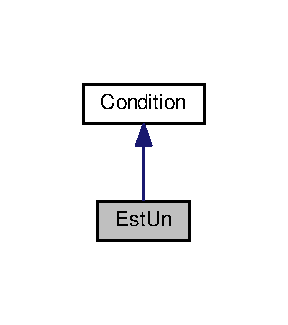
\includegraphics[width=138pt]{class_est_un__coll__graph}
\end{center}
\end{figure}
\subsection*{Public Member Functions}
\begin{DoxyCompactItemize}
\item 
{\bfseries Est\+Un} (const Figure $\ast$f)\hypertarget{class_est_un_af8abb961259349befbbbb9ba9c02f515}{}\label{class_est_un_af8abb961259349befbbbb9ba9c02f515}

\item 
virtual string {\bfseries to\+String} () const \hypertarget{class_est_un_a46a5bd3008a3a45107d5962ee3f781b8}{}\label{class_est_un_a46a5bd3008a3a45107d5962ee3f781b8}

\item 
virtual bool {\bfseries verif} (const Figure $\ast$f) const \hypertarget{class_est_un_a81b052298c0321709280a0097d6f2b8e}{}\label{class_est_un_a81b052298c0321709280a0097d6f2b8e}

\end{DoxyCompactItemize}


\subsection{Detailed Description}
auteurs \+: Michel Landschoot mail \+: \href{mailto:direction@landsnet.com}{\tt direction@landsnet.\+com} date de cr�ation \+: 2013-\/12-\/21 description \+: classe d�crivant la condition \hyperlink{class_est_un}{Est\+Un} 

The documentation for this class was generated from the following file\+:\begin{DoxyCompactItemize}
\item 
archive/est\+Un.\+h\end{DoxyCompactItemize}

\hypertarget{class_et}{}\section{Et Class Reference}
\label{class_et}\index{Et@{Et}}


{\ttfamily \#include $<$et.\+h$>$}



Inheritance diagram for Et\+:
\nopagebreak
\begin{figure}[H]
\begin{center}
\leavevmode
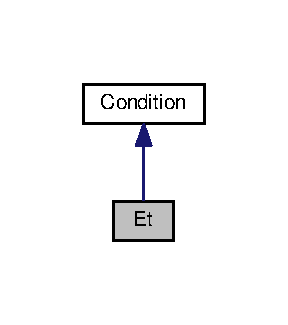
\includegraphics[width=138pt]{class_et__inherit__graph}
\end{center}
\end{figure}


Collaboration diagram for Et\+:
\nopagebreak
\begin{figure}[H]
\begin{center}
\leavevmode
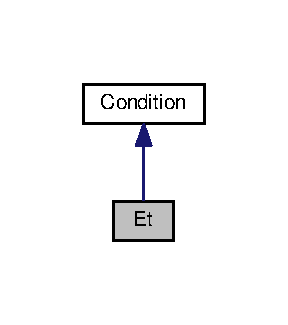
\includegraphics[width=138pt]{class_et__coll__graph}
\end{center}
\end{figure}
\subsection*{Public Member Functions}
\begin{DoxyCompactItemize}
\item 
{\bfseries Et} (\hyperlink{class_condition}{Condition} $\ast$c1, \hyperlink{class_condition}{Condition} $\ast$c2)\hypertarget{class_et_ad4da841742055deac739d32c05b3be7f}{}\label{class_et_ad4da841742055deac739d32c05b3be7f}

\item 
virtual string {\bfseries to\+String} () const \hypertarget{class_et_a292495c84ee5b176515cae63cd854f3b}{}\label{class_et_a292495c84ee5b176515cae63cd854f3b}

\item 
virtual bool {\bfseries verif} (const Figure $\ast$f) const \hypertarget{class_et_a6fb300cddffb467d54c4269baa18a830}{}\label{class_et_a6fb300cddffb467d54c4269baa18a830}

\end{DoxyCompactItemize}


\subsection{Detailed Description}
auteurs \+: Michel Landschoot mail \+: \href{mailto:direction@landsnet.com}{\tt direction@landsnet.\+com} date de cr�ation \+: 2013-\/12-\/21 description \+: classe d�crivant la condition \hyperlink{class_et}{Et}

La classe \hyperlink{class_et}{Et} devrait d�finir un constructeur de copie et une surcharge de l\textquotesingle{}op�rateur =. En effet, elle a 2 attributs de type pointeur. 

The documentation for this class was generated from the following file\+:\begin{DoxyCompactItemize}
\item 
archive/et.\+h\end{DoxyCompactItemize}

\hypertarget{class_filtrage}{}\section{Filtrage Class Reference}
\label{class_filtrage}\index{Filtrage@{Filtrage}}
\subsection*{Static Public Member Functions}
\begin{DoxyCompactItemize}
\item 
static void {\bfseries remplit\+Alea} (list$<$ int $>$ entiers, int n)\hypertarget{class_filtrage_a1a952301ad7adca6815695cd8b411e97}{}\label{class_filtrage_a1a952301ad7adca6815695cd8b411e97}

\item 
static int \hyperlink{class_filtrage_ac574aff99889c49f2a6b81a61f1a0cb5}{compter\+Si} (list$<$ const Figure $\ast$ $>$ figures, \hyperlink{class_condition}{Condition} $\ast$condition, bool test)
\item 
static bool \hyperlink{class_filtrage_a865e8fb6c1fa0725579d983e2b66ef84}{supprimer\+Si} (list$<$ const Figure $\ast$ $>$ \&figures, \hyperlink{class_condition}{Condition} $\ast$condition)
\item 
static bool \hyperlink{class_filtrage_a8811a2bee7d13475c0ab840c9df5b3aa}{supprimer\+Si\+Bis} (list$<$ const Figure $\ast$ $>$ \&figures, \hyperlink{class_condition}{Condition} $\ast$condition)
\item 
static bool \hyperlink{class_filtrage_a3826cecbed118b2c9e35eb341af152e5}{supprimer\+Si\+Profond} (list$<$ const Figure $\ast$ $>$ \&figures, \hyperlink{class_condition}{Condition} $\ast$condition)
\item 
static bool \hyperlink{class_filtrage_a8ccf431f351f1e5b033f0dffc5a12901}{supprimer\+Si\+Profond\+Bis} (list$<$ const Figure $\ast$ $>$ \&figures, \hyperlink{class_condition}{Condition} $\ast$condition)
\item 
static Figure $\ast$ \hyperlink{class_filtrage_ae4db2deedd1ee54a8306cbf5a4c0c82f}{get\+Une\+Figure} (int x, int y)
\item 
static list$<$ const Figure $\ast$ $>$ \hyperlink{class_filtrage_a5feed577946a971f73d22eccfe7c84ba}{creer\+Figures} (int n)
\end{DoxyCompactItemize}


\subsection{Member Function Documentation}
\index{Filtrage@{Filtrage}!compter\+Si@{compter\+Si}}
\index{compter\+Si@{compter\+Si}!Filtrage@{Filtrage}}
\subsubsection[{\texorpdfstring{compter\+Si(list$<$ const Figure $\ast$ $>$ figures, Condition $\ast$condition, bool test)}{compterSi(list< const Figure * > figures, Condition *condition, bool test)}}]{\setlength{\rightskip}{0pt plus 5cm}int Filtrage\+::compter\+Si (
\begin{DoxyParamCaption}
\item[{list$<$ const Figure $\ast$ $>$}]{figures, }
\item[{{\bf Condition} $\ast$}]{condition, }
\item[{bool}]{test}
\end{DoxyParamCaption}
)\hspace{0.3cm}{\ttfamily [static]}}\hypertarget{class_filtrage_ac574aff99889c49f2a6b81a61f1a0cb5}{}\label{class_filtrage_ac574aff99889c49f2a6b81a61f1a0cb5}
retourne le nombre de figures d\textquotesingle{}une liste de figures v�rifiant la condition F\+O\+R\+E\+A\+CH I\+T\+E\+R\+A\+T\+O\+RS\index{Filtrage@{Filtrage}!creer\+Figures@{creer\+Figures}}
\index{creer\+Figures@{creer\+Figures}!Filtrage@{Filtrage}}
\subsubsection[{\texorpdfstring{creer\+Figures(int n)}{creerFigures(int n)}}]{\setlength{\rightskip}{0pt plus 5cm}list$<$ const Figure $\ast$ $>$ Filtrage\+::creer\+Figures (
\begin{DoxyParamCaption}
\item[{int}]{n}
\end{DoxyParamCaption}
)\hspace{0.3cm}{\ttfamily [static]}}\hypertarget{class_filtrage_a5feed577946a971f73d22eccfe7c84ba}{}\label{class_filtrage_a5feed577946a971f73d22eccfe7c84ba}
Utilisation de la S\+TL \+: type list Retourne une liste de figures al�atoires \index{Filtrage@{Filtrage}!get\+Une\+Figure@{get\+Une\+Figure}}
\index{get\+Une\+Figure@{get\+Une\+Figure}!Filtrage@{Filtrage}}
\subsubsection[{\texorpdfstring{get\+Une\+Figure(int x, int y)}{getUneFigure(int x, int y)}}]{\setlength{\rightskip}{0pt plus 5cm}Figure $\ast$ Filtrage\+::get\+Une\+Figure (
\begin{DoxyParamCaption}
\item[{int}]{x, }
\item[{int}]{y}
\end{DoxyParamCaption}
)\hspace{0.3cm}{\ttfamily [static]}}\hypertarget{class_filtrage_ae4db2deedd1ee54a8306cbf5a4c0c82f}{}\label{class_filtrage_ae4db2deedd1ee54a8306cbf5a4c0c82f}
Retourne une figure al�atoire pointeur nul en C++\index{Filtrage@{Filtrage}!supprimer\+Si@{supprimer\+Si}}
\index{supprimer\+Si@{supprimer\+Si}!Filtrage@{Filtrage}}
\subsubsection[{\texorpdfstring{supprimer\+Si(list$<$ const Figure $\ast$ $>$ \&figures, Condition $\ast$condition)}{supprimerSi(list< const Figure * > &figures, Condition *condition)}}]{\setlength{\rightskip}{0pt plus 5cm}bool Filtrage\+::supprimer\+Si (
\begin{DoxyParamCaption}
\item[{list$<$ const Figure $\ast$ $>$ \&}]{figures, }
\item[{{\bf Condition} $\ast$}]{condition}
\end{DoxyParamCaption}
)\hspace{0.3cm}{\ttfamily [static]}}\hypertarget{class_filtrage_a865e8fb6c1fa0725579d983e2b66ef84}{}\label{class_filtrage_a865e8fb6c1fa0725579d983e2b66ef84}
Suppression superficielle des figures satisfaisant la condition supprime les figures de l\textquotesingle{}image en les d�sallouant si la figure est une image alors ses figures sont �galement d�sallou�es Si une image contient une image alors les figures de cette derni�re ne sont pas supprim�es. Utilisation de la m�thode remove ==$>$ utile de copier la liste pour it�rer Les conteneurs g�rent leur structure de donn�es de mani�re dynamique, et sont susceptibles de la r�organiser d�s qu�on les manipule. On veillera donc � ne plus utiliser les it�rateurs d�un conteneur d�s qu�une m�thode permettant de le modifier aura �t� appel�e. Ne pas respecter cette r�gle conduirait, dans le meilleur des cas, � ne pas parcourir compl�tement l�ensemble des objets du conteneur, et dans le pire des cas, � planter imm�diatement le programme

void remove (const value\+\_\+type\& val); The container is modified. The elements removed are modified. Concurrently accessing or modifying other elements is safe, although iterating through the container is not.

==$>$ cr�ation d\textquotesingle{}une copie de la liste l\textquotesingle{}it�ration se fera sur cette copie de liste, et la suppression des �l�ments sur la liste originale

C\+T\+OR de copie superficielle des listes de la S\+TL

F\+O\+R\+E\+A\+CH I\+T\+E\+R\+A\+T\+O\+RS sur la copie

suppression dans la liste originale\index{Filtrage@{Filtrage}!supprimer\+Si\+Bis@{supprimer\+Si\+Bis}}
\index{supprimer\+Si\+Bis@{supprimer\+Si\+Bis}!Filtrage@{Filtrage}}
\subsubsection[{\texorpdfstring{supprimer\+Si\+Bis(list$<$ const Figure $\ast$ $>$ \&figures, Condition $\ast$condition)}{supprimerSiBis(list< const Figure * > &figures, Condition *condition)}}]{\setlength{\rightskip}{0pt plus 5cm}bool Filtrage\+::supprimer\+Si\+Bis (
\begin{DoxyParamCaption}
\item[{list$<$ const Figure $\ast$ $>$ \&}]{figures, }
\item[{{\bf Condition} $\ast$}]{condition}
\end{DoxyParamCaption}
)\hspace{0.3cm}{\ttfamily [static]}}\hypertarget{class_filtrage_a8811a2bee7d13475c0ab840c9df5b3aa}{}\label{class_filtrage_a8811a2bee7d13475c0ab840c9df5b3aa}
Suppression superficielle des figures satisfaisant la condition supprime les figures de l\textquotesingle{}image en les d�sallouant si la figure est une image alors ses figures sont �galement d�sallou�es Si une image contient une image alors les figures de cette derni�re ne sont pas supprim�es. Utilisation de la m�thode erase ==$>$ inutile de copier la liste pour it�rer F\+O\+R\+E\+A\+CH I\+T\+E\+R\+A\+T\+O\+RS

suppression dans la liste originale\index{Filtrage@{Filtrage}!supprimer\+Si\+Profond@{supprimer\+Si\+Profond}}
\index{supprimer\+Si\+Profond@{supprimer\+Si\+Profond}!Filtrage@{Filtrage}}
\subsubsection[{\texorpdfstring{supprimer\+Si\+Profond(list$<$ const Figure $\ast$ $>$ \&figures, Condition $\ast$condition)}{supprimerSiProfond(list< const Figure * > &figures, Condition *condition)}}]{\setlength{\rightskip}{0pt plus 5cm}bool Filtrage\+::supprimer\+Si\+Profond (
\begin{DoxyParamCaption}
\item[{list$<$ const Figure $\ast$ $>$ \&}]{figures, }
\item[{{\bf Condition} $\ast$}]{condition}
\end{DoxyParamCaption}
)\hspace{0.3cm}{\ttfamily [static]}}\hypertarget{class_filtrage_a3826cecbed118b2c9e35eb341af152e5}{}\label{class_filtrage_a3826cecbed118b2c9e35eb341af152e5}
Suppression profonde des figures satisfaisant la condition supprime les figures de l\textquotesingle{}image en les d�sallouant si la figure est une image alors ses figures sont �galement d�sallou�es si une image contient une image alors les figures de cette derni�re sont supprim�es. Utilisation de la m�thode remove ==$>$ utile de copier la liste pour it�rer \index{Filtrage@{Filtrage}!supprimer\+Si\+Profond\+Bis@{supprimer\+Si\+Profond\+Bis}}
\index{supprimer\+Si\+Profond\+Bis@{supprimer\+Si\+Profond\+Bis}!Filtrage@{Filtrage}}
\subsubsection[{\texorpdfstring{supprimer\+Si\+Profond\+Bis(list$<$ const Figure $\ast$ $>$ \&figures, Condition $\ast$condition)}{supprimerSiProfondBis(list< const Figure * > &figures, Condition *condition)}}]{\setlength{\rightskip}{0pt plus 5cm}bool Filtrage\+::supprimer\+Si\+Profond\+Bis (
\begin{DoxyParamCaption}
\item[{list$<$ const Figure $\ast$ $>$ \&}]{figures, }
\item[{{\bf Condition} $\ast$}]{condition}
\end{DoxyParamCaption}
)\hspace{0.3cm}{\ttfamily [static]}}\hypertarget{class_filtrage_a8ccf431f351f1e5b033f0dffc5a12901}{}\label{class_filtrage_a8ccf431f351f1e5b033f0dffc5a12901}
Suppression profonde des figures satisfaisant la condition supprime les figures de l\textquotesingle{}image en les d�sallouant si la figure est une image alors ses figures sont �galement d�sallou�es si une image contient une image alors les figures de cette derni�re sont supprim�es. Utilisation de la m�thode erase ==$>$ inutile de copier la liste pour it�rer F\+O\+R\+E\+A\+CH I\+T\+E\+R\+A\+T\+O\+RS

succ�s du dynamic-\/cast \+: on a une image

suppression de l\textquotesingle{}image

Insertion des figures de l\textquotesingle{}image qui ne satisfont pas la condition dans une nouvelle image Puis insertion de cette nouvelle image dans la liste des figures.

insertion en t�te afin d\textquotesingle{}�viter que l\textquotesingle{}it�rateur devienne incoh�rent

The documentation for this class was generated from the following files\+:\begin{DoxyCompactItemize}
\item 
archive/filtrage.\+h\item 
archive/filtrage.\+cpp\end{DoxyCompactItemize}

\hypertarget{class_image}{}\section{Image Class Reference}
\label{class_image}\index{Image@{Image}}


{\ttfamily \#include $<$image.\+hpp$>$}



Inheritance diagram for Image\+:
\nopagebreak
\begin{figure}[H]
\begin{center}
\leavevmode
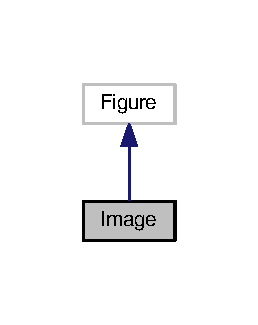
\includegraphics[width=124pt]{class_image__inherit__graph}
\end{center}
\end{figure}


Collaboration diagram for Image\+:
\nopagebreak
\begin{figure}[H]
\begin{center}
\leavevmode
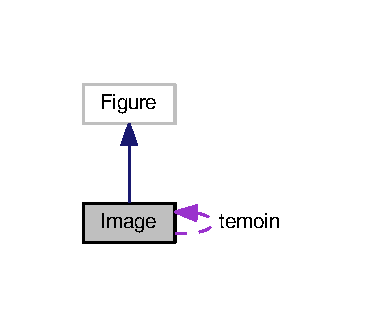
\includegraphics[width=175pt]{class_image__coll__graph}
\end{center}
\end{figure}
\subsection*{Public Types}
\begin{DoxyCompactItemize}
\item 
enum \{ {\bfseries I\+M\+A\+G\+E\+\_\+\+M\+AX} = 50
 \}\hypertarget{class_image_a1d78dd24522ac145e075f5fd6aad5067}{}\label{class_image_a1d78dd24522ac145e075f5fd6aad5067}

\end{DoxyCompactItemize}
\subsection*{Public Member Functions}
\begin{DoxyCompactItemize}
\item 
{\bfseries Image} (const \hyperlink{class_point}{Point} \&a=\hyperlink{class_point}{Point}(0, 0))\hypertarget{class_image_a054df7fc4b3ac77b15cac04599af8213}{}\label{class_image_a054df7fc4b3ac77b15cac04599af8213}

\item 
\hyperlink{class_image_a34410a36b132ab597a8878d45facc89a}{Image} (const \hyperlink{class_image}{Image} \&image)
\item 
virtual Figure $\ast$ \hyperlink{class_image_ae80b4ae48c105f76b7d142e12c4bf3dc}{copy} () const 
\item 
virtual \hyperlink{class_image_a46561cd7dcf7e203e9579737e8ace4eb}{$\sim$\+Image} ()
\item 
Figure $\ast$ {\bfseries get\+Figure} (int index) const \hypertarget{class_image_a18b25740f2082c2f4095f4738c839997}{}\label{class_image_a18b25740f2082c2f4095f4738c839997}

\item 
void {\bfseries set\+Figure} (int index, Figure $\ast$figure)\hypertarget{class_image_a1051bd8ae63eabeeeb6f37aa048c15e6}{}\label{class_image_a1051bd8ae63eabeeeb6f37aa048c15e6}

\item 
int {\bfseries get\+Nombre} () const \hypertarget{class_image_a2b0813ba90870ac3cfae515406cd5afc}{}\label{class_image_a2b0813ba90870ac3cfae515406cd5afc}

\item 
\hyperlink{class_point}{Point} {\bfseries get\+Origine} () const \hypertarget{class_image_ac057ace4fea5e06b71eb6996cc49ec02}{}\label{class_image_ac057ace4fea5e06b71eb6996cc49ec02}

\item 
void \hyperlink{class_image_acac393f8fe4d375f1d7ca2340517824b}{ajouter} (const Figure \&f)
\item 
virtual list$<$ \hyperlink{class_point}{Point} $\ast$ $>$ {\bfseries get\+Points} () const \hypertarget{class_image_a263966190234ac1c38a716356f529b2e}{}\label{class_image_a263966190234ac1c38a716356f529b2e}

\item 
virtual void \hyperlink{class_image_a50ead8205b30251a11a98da86ad1bfad}{deplacer} (const \hyperlink{class_point}{Point} \&trans)
\item 
virtual void \hyperlink{class_image_a4f2367997cf04d6d9f104178075b8d44}{dessiner} (ostream \&os=cout) const 
\item 
virtual double {\bfseries surface} () const \hypertarget{class_image_a735711df9697beb868ccb9dd1dfce0fb}{}\label{class_image_a735711df9697beb868ccb9dd1dfce0fb}

\item 
virtual double {\bfseries perimetre} () const \hypertarget{class_image_a6bcc6b782428b4407fa26dab32f05d34}{}\label{class_image_a6bcc6b782428b4407fa26dab32f05d34}

\item 
virtual double {\bfseries distance\+\_\+origine} (const \hyperlink{class_point}{Point} \&p) const \hypertarget{class_image_af2533395749e8976cab616a65cf512d1}{}\label{class_image_af2533395749e8976cab616a65cf512d1}

\item 
virtual void {\bfseries afficher} (ostream \&os=cout) const \hypertarget{class_image_a3d26f1178af2563a90b51ad1babe8ee0}{}\label{class_image_a3d26f1178af2563a90b51ad1babe8ee0}

\end{DoxyCompactItemize}
\subsection*{Static Public Attributes}
\begin{DoxyCompactItemize}
\item 
static \hyperlink{class_image}{Image} \hyperlink{class_image_a19d374f4783eaa0126721ac0c4d472c8}{temoin} = \hyperlink{class_image}{Image}()
\end{DoxyCompactItemize}


\subsection{Detailed Description}
Politique uniforme d\textquotesingle{}allocation m�moire Toutes les figures sont allou�es dynamiquement Une image les m�morise via un tableau de pointeurs de figures 

\subsection{Constructor \& Destructor Documentation}
\index{Image@{Image}!Image@{Image}}
\index{Image@{Image}!Image@{Image}}
\subsubsection[{\texorpdfstring{Image(const Image \&image)}{Image(const Image &image)}}]{\setlength{\rightskip}{0pt plus 5cm}Image\+::\+Image (
\begin{DoxyParamCaption}
\item[{const {\bf Image} \&}]{image}
\end{DoxyParamCaption}
)}\hypertarget{class_image_a34410a36b132ab597a8878d45facc89a}{}\label{class_image_a34410a36b132ab597a8878d45facc89a}
contructeur de copie profonde \index{Image@{Image}!````~Image@{$\sim$\+Image}}
\index{````~Image@{$\sim$\+Image}!Image@{Image}}
\subsubsection[{\texorpdfstring{$\sim$\+Image()}{~Image()}}]{\setlength{\rightskip}{0pt plus 5cm}virtual Image\+::$\sim$\+Image (
\begin{DoxyParamCaption}
{}
\end{DoxyParamCaption}
)\hspace{0.3cm}{\ttfamily [inline]}, {\ttfamily [virtual]}}\hypertarget{class_image_a46561cd7dcf7e203e9579737e8ace4eb}{}\label{class_image_a46561cd7dcf7e203e9579737e8ace4eb}
B\+UG si partage d\textquotesingle{}instances allou�es dynamiquement ==$>$ IL F\+A\+UT I\+M\+P\+L\+E\+M\+E\+N\+T\+ER D\+ES C\+O\+M\+P\+T\+E\+U\+RS DE R\+E\+F\+E\+R\+E\+N\+C\+ES Dans l\textquotesingle{}impl�mentation propos�e, les instances sont recopi�es lorsqu\textquotesingle{}elles sont ajout�es dans le tableau de figures. Il n\textquotesingle{}y a pas de partage d\textquotesingle{}instances. Dans la m�thode ajouter on a \+: \+\_\+tableau\mbox{[}\+\_\+nombre++\mbox{]} = ((Figure $\ast$) \&f)-\/$>$\hyperlink{class_image_ae80b4ae48c105f76b7d142e12c4bf3dc}{copy()};

\subsection{Member Function Documentation}
\index{Image@{Image}!ajouter@{ajouter}}
\index{ajouter@{ajouter}!Image@{Image}}
\subsubsection[{\texorpdfstring{ajouter(const Figure \&f)}{ajouter(const Figure &f)}}]{\setlength{\rightskip}{0pt plus 5cm}void Image\+::ajouter (
\begin{DoxyParamCaption}
\item[{const Figure \&}]{f}
\end{DoxyParamCaption}
)}\hypertarget{class_image_acac393f8fe4d375f1d7ca2340517824b}{}\label{class_image_acac393f8fe4d375f1d7ca2340517824b}
ajout d\textquotesingle{} une figure � une image Code pour du partage d\textquotesingle{}instances allou�es dynamiquement n�cessite des compteurs de r�f�rence pour leur lib�ration m�moire en C ==$>$ A\+B\+A\+N\+D\+ON \+\_\+tableau\mbox{[}\+\_\+nombre++\mbox{]} = (Figure $\ast$) (\&f); en C++\+: du const\+\_\+cast \+\_\+tableau\mbox{[}\+\_\+nombre++\mbox{]} = const\+\_\+cast$<$\+Figure $\ast$$>$ (\&f);\index{Image@{Image}!copy@{copy}}
\index{copy@{copy}!Image@{Image}}
\subsubsection[{\texorpdfstring{copy() const }{copy() const }}]{\setlength{\rightskip}{0pt plus 5cm}Figure $\ast$ Image\+::copy (
\begin{DoxyParamCaption}
{}
\end{DoxyParamCaption}
) const\hspace{0.3cm}{\ttfamily [virtual]}}\hypertarget{class_image_ae80b4ae48c105f76b7d142e12c4bf3dc}{}\label{class_image_ae80b4ae48c105f76b7d142e12c4bf3dc}
Fonction virtuelle de copie \index{Image@{Image}!deplacer@{deplacer}}
\index{deplacer@{deplacer}!Image@{Image}}
\subsubsection[{\texorpdfstring{deplacer(const Point \&trans)}{deplacer(const Point &trans)}}]{\setlength{\rightskip}{0pt plus 5cm}void Image\+::deplacer (
\begin{DoxyParamCaption}
\item[{const {\bf Point} \&}]{p}
\end{DoxyParamCaption}
)\hspace{0.3cm}{\ttfamily [virtual]}}\hypertarget{class_image_a50ead8205b30251a11a98da86ad1bfad}{}\label{class_image_a50ead8205b30251a11a98da86ad1bfad}
D�placement-\/translation de valeur le point p toutes les figures de l\textquotesingle{}image sont �galement d�plac�es \index{Image@{Image}!dessiner@{dessiner}}
\index{dessiner@{dessiner}!Image@{Image}}
\subsubsection[{\texorpdfstring{dessiner(ostream \&os=cout) const }{dessiner(ostream &os=cout) const }}]{\setlength{\rightskip}{0pt plus 5cm}void Image\+::dessiner (
\begin{DoxyParamCaption}
\item[{ostream \&}]{os = {\ttfamily cout}}
\end{DoxyParamCaption}
) const\hspace{0.3cm}{\ttfamily [virtual]}}\hypertarget{class_image_a4f2367997cf04d6d9f104178075b8d44}{}\label{class_image_a4f2367997cf04d6d9f104178075b8d44}
Le dessin se limite � un affichage 

\subsection{Member Data Documentation}
\index{Image@{Image}!temoin@{temoin}}
\index{temoin@{temoin}!Image@{Image}}
\subsubsection[{\texorpdfstring{temoin}{temoin}}]{\setlength{\rightskip}{0pt plus 5cm}{\bf Image} Image\+::temoin = {\bf Image}()\hspace{0.3cm}{\ttfamily [static]}}\hypertarget{class_image_a19d374f4783eaa0126721ac0c4d472c8}{}\label{class_image_a19d374f4783eaa0126721ac0c4d472c8}
L\textquotesingle{}image t�moin est une variable de classe 

The documentation for this class was generated from the following files\+:\begin{DoxyCompactItemize}
\item 
archive/image.\+hpp\item 
archive/image.\+cpp\end{DoxyCompactItemize}

\hypertarget{class_line}{}\section{Line Class Reference}
\label{class_line}\index{Line@{Line}}


{\ttfamily \#include $<$Line.\+hpp$>$}



Inheritance diagram for Line\+:
\nopagebreak
\begin{figure}[H]
\begin{center}
\leavevmode
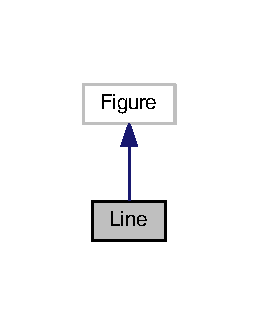
\includegraphics[width=124pt]{class_line__inherit__graph}
\end{center}
\end{figure}


Collaboration diagram for Line\+:
\nopagebreak
\begin{figure}[H]
\begin{center}
\leavevmode
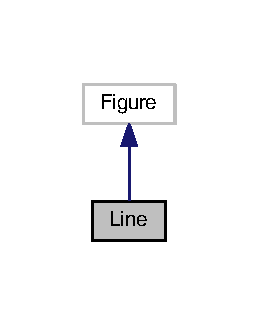
\includegraphics[width=124pt]{class_line__coll__graph}
\end{center}
\end{figure}
\subsection*{Public Member Functions}
\begin{DoxyCompactItemize}
\item 
{\bfseries Line} (const \hyperlink{class_point}{Point} \&a, const \hyperlink{class_point}{Point} \&b)\hypertarget{class_line_a0ec34f80a43014768ec228bfa87fd15f}{}\label{class_line_a0ec34f80a43014768ec228bfa87fd15f}

\item 
virtual \hyperlink{class_line}{Line} $\ast$ \hyperlink{class_line_a47eb8ca4b98da5903b2e781bf6feeeb4}{copy} () const 
\begin{DoxyCompactList}\small\item\em Fonction virtuelle de copie. \end{DoxyCompactList}\item 
\hyperlink{class_point}{Point} {\bfseries get\+Origin} () const \hypertarget{class_line_ad75b05eb47a8701b3e997a731c093b29}{}\label{class_line_ad75b05eb47a8701b3e997a731c093b29}

\item 
\hyperlink{class_point}{Point} {\bfseries get\+Extremity} () const \hypertarget{class_line_a223ea932601e8ed5c4e2278e67f09fc3}{}\label{class_line_a223ea932601e8ed5c4e2278e67f09fc3}

\item 
virtual void \hyperlink{class_line_a1b8116c3c461dbb207f927f9e244fd9f}{translation} (const \hyperlink{class_point}{Point} \&p)
\item 
virtual void {\bfseries homothety} (const \hyperlink{class_point}{Point} \&p)\hypertarget{class_line_ae9acdfb8611ad7af187ad908fa3323f6}{}\label{class_line_ae9acdfb8611ad7af187ad908fa3323f6}

\item 
virtual void {\bfseries rotation} (const double radius)\hypertarget{class_line_aa61b4ecedc27f78a24192b5e44b7c2c0}{}\label{class_line_aa61b4ecedc27f78a24192b5e44b7c2c0}

\item 
virtual void {\bfseries central\+Symmetry} (initializer\+\_\+list$<$ \hyperlink{class_point}{Point} $>$ \&p)\hypertarget{class_line_a3724edda57b9095ce0af7c5a73379387}{}\label{class_line_a3724edda57b9095ce0af7c5a73379387}

\item 
virtual void {\bfseries axial\+SymmetryX} (initializer\+\_\+list$<$ \hyperlink{class_point}{Point} $>$ \&p)\hypertarget{class_line_acde0f7b21fd12feed799721d6bc57d17}{}\label{class_line_acde0f7b21fd12feed799721d6bc57d17}

\item 
virtual void {\bfseries axial\+SymmetryY} (initializer\+\_\+list$<$ \hyperlink{class_point}{Point} $>$ \&p)\hypertarget{class_line_a5dfdfd77686b63d0d9f8ab641d305867}{}\label{class_line_a5dfdfd77686b63d0d9f8ab641d305867}

\item 
virtual void {\bfseries draw} (ostream \&os=cout) const \hypertarget{class_line_a76dd03f158c3ff373dff29920eaccb81}{}\label{class_line_a76dd03f158c3ff373dff29920eaccb81}

\item 
virtual void {\bfseries print} (ostream \&os=cout) const \hypertarget{class_line_a97980f6509664d801e433590116d9c93}{}\label{class_line_a97980f6509664d801e433590116d9c93}

\item 
virtual double \hyperlink{class_line_ae531ddee8ae3446429c9078b4a8a51a9}{surface} () const 
\item 
virtual double {\bfseries perimeter} () const \hypertarget{class_line_af45d5df18885aa3e3f17a3f771add167}{}\label{class_line_af45d5df18885aa3e3f17a3f771add167}

\item 
virtual double {\bfseries origine\+Distance} (const \hyperlink{class_point}{Point} \&p) const \hypertarget{class_line_ad78622905b4960d4e576959d55e39bd1}{}\label{class_line_ad78622905b4960d4e576959d55e39bd1}

\end{DoxyCompactItemize}
\subsection*{Static Public Attributes}
\begin{DoxyCompactItemize}
\item 
static Ligne \hyperlink{class_line_a24d84e551f2ffcfda32fcc2ca66c9f76}{temoin} = \hyperlink{class_line}{Line}(\hyperlink{class_point}{Point}(0,0), \hyperlink{class_point}{Point}(1,1))
\end{DoxyCompactItemize}


\subsection{Detailed Description}
auteurs \+: Michel Landschoot mail \+: \href{mailto:direction@landsnet.com}{\tt direction@landsnet.\+com} date de cr�ation \+: 2013-\/12-\/21 description \+: classe d�crivant une ligne dans une hi�rachie de figures 

\subsection{Member Function Documentation}
\index{Line@{Line}!copy@{copy}}
\index{copy@{copy}!Line@{Line}}
\subsubsection[{\texorpdfstring{copy() const }{copy() const }}]{\setlength{\rightskip}{0pt plus 5cm}Figure $\ast$ Line\+::copy (
\begin{DoxyParamCaption}
{}
\end{DoxyParamCaption}
) const\hspace{0.3cm}{\ttfamily [virtual]}}\hypertarget{class_line_a47eb8ca4b98da5903b2e781bf6feeeb4}{}\label{class_line_a47eb8ca4b98da5903b2e781bf6feeeb4}


Fonction virtuelle de copie. 


\begin{DoxyParams}{Parameters}
{\em } & \\
\hline
\end{DoxyParams}
\index{Line@{Line}!surface@{surface}}
\index{surface@{surface}!Line@{Line}}
\subsubsection[{\texorpdfstring{surface() const }{surface() const }}]{\setlength{\rightskip}{0pt plus 5cm}double Line\+::surface (
\begin{DoxyParamCaption}
{}
\end{DoxyParamCaption}
) const\hspace{0.3cm}{\ttfamily [virtual]}}\hypertarget{class_line_ae531ddee8ae3446429c9078b4a8a51a9}{}\label{class_line_ae531ddee8ae3446429c9078b4a8a51a9}
T\+O\+UR DE M\+A\+G\+IE G\+E\+O\+M\+E\+T\+R\+I\+Q\+UE une ligne est vue pour les besoins de la cause comme une segment (origine, exptremite\mbox{]} avec une �paisseur soit un rectangle dont on peut calculer la surfade!!!! \index{Line@{Line}!translation@{translation}}
\index{translation@{translation}!Line@{Line}}
\subsubsection[{\texorpdfstring{translation(const Point \&p)}{translation(const Point &p)}}]{\setlength{\rightskip}{0pt plus 5cm}void Line\+::translation (
\begin{DoxyParamCaption}
\item[{const {\bf Point} \&}]{p}
\end{DoxyParamCaption}
)\hspace{0.3cm}{\ttfamily [virtual]}}\hypertarget{class_line_a1b8116c3c461dbb207f927f9e244fd9f}{}\label{class_line_a1b8116c3c461dbb207f927f9e244fd9f}
D�placement-\/translation de valeur le point p 

\subsection{Member Data Documentation}
\index{Line@{Line}!temoin@{temoin}}
\index{temoin@{temoin}!Line@{Line}}
\subsubsection[{\texorpdfstring{temoin}{temoin}}]{\setlength{\rightskip}{0pt plus 5cm}{\bf Line} Line\+::temoin = {\bf Line}({\bf Point}(0,0), {\bf Point}(1,1))\hspace{0.3cm}{\ttfamily [static]}}\hypertarget{class_line_a24d84e551f2ffcfda32fcc2ca66c9f76}{}\label{class_line_a24d84e551f2ffcfda32fcc2ca66c9f76}
La ligne t�moin est une variable de classe 

The documentation for this class was generated from the following files\+:\begin{DoxyCompactItemize}
\item 
include/Line.\+hpp\item 
src/\hyperlink{_line_8cpp}{Line.\+cpp}\end{DoxyCompactItemize}

\hypertarget{class_matrice2_d}{}\section{Matrice2D Class Reference}
\label{class_matrice2_d}\index{Matrice2D@{Matrice2D}}
\subsection*{Friends}
\begin{DoxyCompactItemize}
\item 
void {\bfseries translation} (const \hyperlink{class_point}{Point} \&p, Figure \&figure)\hypertarget{class_matrice2_d_a4384bd2f5dcd6120136ea610c770feed}{}\label{class_matrice2_d_a4384bd2f5dcd6120136ea610c770feed}

\item 
void {\bfseries homothety} (const \hyperlink{class_point}{Point} \&p, Figure \&figure)\hypertarget{class_matrice2_d_abc140d30a77cbba53aec8fa763f4e303}{}\label{class_matrice2_d_abc140d30a77cbba53aec8fa763f4e303}

\item 
void {\bfseries rotation} (const double angle, initializer\+\_\+list$<$ \hyperlink{class_point}{Point} $>$ \&p)\hypertarget{class_matrice2_d_ae7cf79117e4afdc89342479115362113}{}\label{class_matrice2_d_ae7cf79117e4afdc89342479115362113}

\item 
void {\bfseries axial\+SymmetryX} (initializer\+\_\+list$<$ \hyperlink{class_point}{Point} $>$ \&p)\hypertarget{class_matrice2_d_a3e79dbd15ee80d3349565c0cd6ac4142}{}\label{class_matrice2_d_a3e79dbd15ee80d3349565c0cd6ac4142}

\item 
void {\bfseries axial\+SymmetryY} (initializer\+\_\+list$<$ \hyperlink{class_point}{Point} $>$ \&p)\hypertarget{class_matrice2_d_ad7251cd751be521a61467913a841f29f}{}\label{class_matrice2_d_ad7251cd751be521a61467913a841f29f}

\item 
void {\bfseries central\+Symmetry} (initializer\+\_\+list$<$ \hyperlink{class_point}{Point} $>$ \&p)\hypertarget{class_matrice2_d_ae6b975104b9c27e7a7586fa1515ac2d0}{}\label{class_matrice2_d_ae6b975104b9c27e7a7586fa1515ac2d0}

\end{DoxyCompactItemize}


The documentation for this class was generated from the following files\+:\begin{DoxyCompactItemize}
\item 
include/Matrice2\+D.\+hpp\item 
src/Matrice2\+D.\+cpp\end{DoxyCompactItemize}

\hypertarget{class_non}{}\section{Non Class Reference}
\label{class_non}\index{Non@{Non}}


{\ttfamily \#include $<$non.\+h$>$}



Inheritance diagram for Non\+:
\nopagebreak
\begin{figure}[H]
\begin{center}
\leavevmode
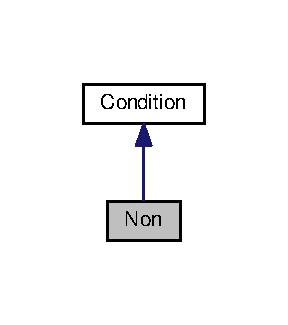
\includegraphics[width=138pt]{class_non__inherit__graph}
\end{center}
\end{figure}


Collaboration diagram for Non\+:
\nopagebreak
\begin{figure}[H]
\begin{center}
\leavevmode
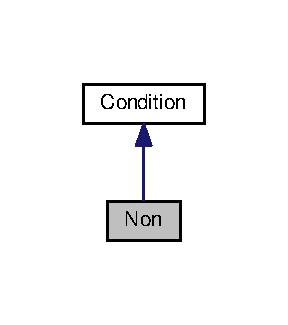
\includegraphics[width=138pt]{class_non__coll__graph}
\end{center}
\end{figure}
\subsection*{Public Member Functions}
\begin{DoxyCompactItemize}
\item 
{\bfseries Non} (\hyperlink{class_condition}{Condition} $\ast$c)\hypertarget{class_non_af2f5620de86ea14adbeaa156d4ab4784}{}\label{class_non_af2f5620de86ea14adbeaa156d4ab4784}

\item 
virtual string {\bfseries to\+String} () const \hypertarget{class_non_a780a2d005b544469b8f6b339af408b2f}{}\label{class_non_a780a2d005b544469b8f6b339af408b2f}

\item 
virtual bool {\bfseries verif} (const Figure $\ast$f) const \hypertarget{class_non_a046168d5d71e0329da28423de806727f}{}\label{class_non_a046168d5d71e0329da28423de806727f}

\end{DoxyCompactItemize}


\subsection{Detailed Description}
auteurs \+: Michel Landschoot mail \+: \href{mailto:direction@landsnet.com}{\tt direction@landsnet.\+com} date de cr�ation \+: 2013-\/12-\/21 description \+: classe d�crivant la condition \hyperlink{class_non}{Non}

La classe \hyperlink{class_non}{Non} devrait d�finir un constructeur de copie et une surcharge de l\textquotesingle{}op�rateur =. En effet, elle a un attribut de type pointeur. 

The documentation for this class was generated from the following file\+:\begin{DoxyCompactItemize}
\item 
archive/non.\+h\end{DoxyCompactItemize}

\hypertarget{class_point}{}\section{Point Class Reference}
\label{class_point}\index{Point@{Point}}
\subsection*{Public Member Functions}
\begin{DoxyCompactItemize}
\item 
\hyperlink{class_point_a9f2d92aa1413f85c7d0e0ff44cd472dc}{Point} (int a=0, int b=0)
\item 
int {\bfseries getX} () const \hypertarget{class_point_abe622fffc8785b0c2e06cdac681b9837}{}\label{class_point_abe622fffc8785b0c2e06cdac681b9837}

\item 
void {\bfseries setX} (int a)\hypertarget{class_point_af1d7384048c7917946feac28371d1b48}{}\label{class_point_af1d7384048c7917946feac28371d1b48}

\item 
int {\bfseries getY} () const \hypertarget{class_point_a10f31e48e2dbc22e3660ca769b8d5d65}{}\label{class_point_a10f31e48e2dbc22e3660ca769b8d5d65}

\item 
void {\bfseries setY} (int b)\hypertarget{class_point_ab12d000e6ccd1bd5ce9a7dc7ea12ef0e}{}\label{class_point_ab12d000e6ccd1bd5ce9a7dc7ea12ef0e}

\item 
\hyperlink{class_point}{Point} {\bfseries operator+} (const \hyperlink{class_point}{Point} \&p) const \hypertarget{class_point_a78421c6bc6fe671fa5ee80e99c0b7284}{}\label{class_point_a78421c6bc6fe671fa5ee80e99c0b7284}

\item 
\hyperlink{class_point}{Point} \& {\bfseries operator+=} (const \hyperlink{class_point}{Point} \&p)\hypertarget{class_point_ae25b726a057b78fd66bdf470b2c79f44}{}\label{class_point_ae25b726a057b78fd66bdf470b2c79f44}

\item 
\hyperlink{class_point}{Point} \& {\bfseries operator=} (const \hyperlink{class_point}{Point} \&p)\hypertarget{class_point_a38ec052f1f90418e9266a1fecf8f9e6e}{}\label{class_point_a38ec052f1f90418e9266a1fecf8f9e6e}

\end{DoxyCompactItemize}
\subsection*{Friends}
\begin{DoxyCompactItemize}
\item 
ostream \& {\bfseries operator$<$$<$} (ostream \&os, const \hyperlink{class_point}{Point} \&p)\hypertarget{class_point_a16c222f303e4df1add09f03a1626f9e9}{}\label{class_point_a16c222f303e4df1add09f03a1626f9e9}

\end{DoxyCompactItemize}


\subsection{Constructor \& Destructor Documentation}
\index{Point@{Point}!Point@{Point}}
\index{Point@{Point}!Point@{Point}}
\subsubsection[{\texorpdfstring{Point(int a=0, int b=0)}{Point(int a=0, int b=0)}}]{\setlength{\rightskip}{0pt plus 5cm}Point\+::\+Point (
\begin{DoxyParamCaption}
\item[{int}]{a = {\ttfamily 0}, }
\item[{int}]{b = {\ttfamily 0}}
\end{DoxyParamCaption}
)}\hypertarget{class_point_a9f2d92aa1413f85c7d0e0ff44cd472dc}{}\label{class_point_a9f2d92aa1413f85c7d0e0ff44cd472dc}
auteurs \+: Michel Landschoot mail \+: \href{mailto:direction@landsnet.com}{\tt direction@landsnet.\+com} date de cr�ation \+: 2013-\/12-\/21 description \+: impl�m�ntation d\textquotesingle{}une classe d�crivant un point 

The documentation for this class was generated from the following files\+:\begin{DoxyCompactItemize}
\item 
include/Point.\+hpp\item 
src/Point.\+cpp\end{DoxyCompactItemize}

\hypertarget{class_rectangle}{}\section{Rectangle Class Reference}
\label{class_rectangle}\index{Rectangle@{Rectangle}}


Inheritance diagram for Rectangle\+:
\nopagebreak
\begin{figure}[H]
\begin{center}
\leavevmode
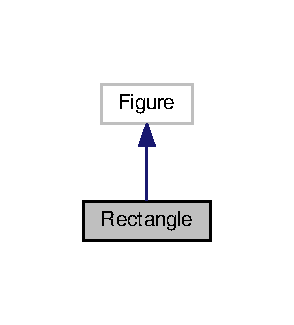
\includegraphics[width=141pt]{class_rectangle__inherit__graph}
\end{center}
\end{figure}


Collaboration diagram for Rectangle\+:
\nopagebreak
\begin{figure}[H]
\begin{center}
\leavevmode
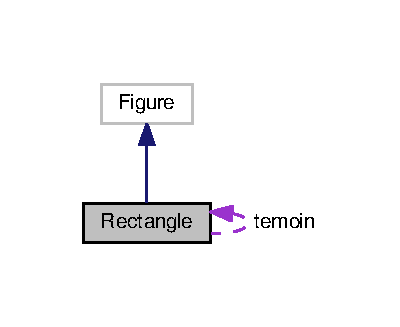
\includegraphics[width=192pt]{class_rectangle__coll__graph}
\end{center}
\end{figure}
\subsection*{Public Member Functions}
\begin{DoxyCompactItemize}
\item 
{\bfseries Rectangle} (const \hyperlink{class_point}{Point} \&a, const \hyperlink{class_point}{Point} \&b)\hypertarget{class_rectangle_a624f003522cefccbf7d7cbbb25484319}{}\label{class_rectangle_a624f003522cefccbf7d7cbbb25484319}

\item 
\hyperlink{class_point}{Point} {\bfseries getA} () const \hypertarget{class_rectangle_a2f4d4c5ae1fa57ffc1fd1db3edcd00b1}{}\label{class_rectangle_a2f4d4c5ae1fa57ffc1fd1db3edcd00b1}

\item 
\hyperlink{class_point}{Point} {\bfseries getB} () const \hypertarget{class_rectangle_ab50635c7b64c91fc6a68890db61bfae6}{}\label{class_rectangle_ab50635c7b64c91fc6a68890db61bfae6}

\item 
\hyperlink{class_point}{Point} {\bfseries getC} () const \hypertarget{class_rectangle_a5339db7a9327c904ccc6df350212cac4}{}\label{class_rectangle_a5339db7a9327c904ccc6df350212cac4}

\item 
\hyperlink{class_point}{Point} {\bfseries getD} () const \hypertarget{class_rectangle_a10f2ecee98b54ac6d9b23a15449a1bd5}{}\label{class_rectangle_a10f2ecee98b54ac6d9b23a15449a1bd5}

\item 
virtual Figure $\ast$ \hyperlink{class_rectangle_a79aa738432ccb76ac84173bec4c31b7c}{copy} () const 
\item 
virtual list$<$ \hyperlink{class_point}{Point} $\ast$ $>$ {\bfseries get\+Points} () const \hypertarget{class_rectangle_a0db01df72e63eebc2c175f58f966cf94}{}\label{class_rectangle_a0db01df72e63eebc2c175f58f966cf94}

\item 
virtual void \hyperlink{class_rectangle_acfa7c56f2c0a087e908c4f7bc542c826}{deplacer} (const \hyperlink{class_point}{Point} \&trans)
\item 
virtual void \hyperlink{class_rectangle_a853147554cb4938530f75f83cf43b6c4}{dessiner} (ostream \&os=cout) const 
\item 
virtual double \hyperlink{class_rectangle_ac2ecb396e91ee632188df53c2322fbef}{surface} () const 
\item 
virtual double {\bfseries perimetre} () const \hypertarget{class_rectangle_ad01dd31ee53ad6920cd126382bb09b90}{}\label{class_rectangle_ad01dd31ee53ad6920cd126382bb09b90}

\item 
virtual double {\bfseries distance\+\_\+origine} (const \hyperlink{class_point}{Point} \&p) const \hypertarget{class_rectangle_a72cf6d5bada2e80849c7bf457ad086f2}{}\label{class_rectangle_a72cf6d5bada2e80849c7bf457ad086f2}

\item 
virtual void {\bfseries afficher} (ostream \&os=cout) const \hypertarget{class_rectangle_a3d9297623b84cf6c94cbc952be511003}{}\label{class_rectangle_a3d9297623b84cf6c94cbc952be511003}

\end{DoxyCompactItemize}
\subsection*{Static Public Attributes}
\begin{DoxyCompactItemize}
\item 
static \hyperlink{class_rectangle}{Rectangle} \hyperlink{class_rectangle_a231d88467ce5857f7546e20bef46ed2c}{temoin} = \hyperlink{class_rectangle}{Rectangle}(\hyperlink{class_point}{Point}(0,0), \hyperlink{class_point}{Point}(2,2))
\end{DoxyCompactItemize}


\subsection{Member Function Documentation}
\index{Rectangle@{Rectangle}!copy@{copy}}
\index{copy@{copy}!Rectangle@{Rectangle}}
\subsubsection[{\texorpdfstring{copy() const }{copy() const }}]{\setlength{\rightskip}{0pt plus 5cm}Figure $\ast$ Rectangle\+::copy (
\begin{DoxyParamCaption}
{}
\end{DoxyParamCaption}
) const\hspace{0.3cm}{\ttfamily [virtual]}}\hypertarget{class_rectangle_a79aa738432ccb76ac84173bec4c31b7c}{}\label{class_rectangle_a79aa738432ccb76ac84173bec4c31b7c}
Fonction virtuelle de copie \index{Rectangle@{Rectangle}!deplacer@{deplacer}}
\index{deplacer@{deplacer}!Rectangle@{Rectangle}}
\subsubsection[{\texorpdfstring{deplacer(const Point \&trans)}{deplacer(const Point &trans)}}]{\setlength{\rightskip}{0pt plus 5cm}void Rectangle\+::deplacer (
\begin{DoxyParamCaption}
\item[{const {\bf Point} \&}]{p}
\end{DoxyParamCaption}
)\hspace{0.3cm}{\ttfamily [virtual]}}\hypertarget{class_rectangle_acfa7c56f2c0a087e908c4f7bc542c826}{}\label{class_rectangle_acfa7c56f2c0a087e908c4f7bc542c826}
Déplacement-\/translation de valeur le point p \index{Rectangle@{Rectangle}!dessiner@{dessiner}}
\index{dessiner@{dessiner}!Rectangle@{Rectangle}}
\subsubsection[{\texorpdfstring{dessiner(ostream \&os=cout) const }{dessiner(ostream &os=cout) const }}]{\setlength{\rightskip}{0pt plus 5cm}void Rectangle\+::dessiner (
\begin{DoxyParamCaption}
\item[{ostream \&}]{os = {\ttfamily cout}}
\end{DoxyParamCaption}
) const\hspace{0.3cm}{\ttfamily [virtual]}}\hypertarget{class_rectangle_a853147554cb4938530f75f83cf43b6c4}{}\label{class_rectangle_a853147554cb4938530f75f83cf43b6c4}
Le dessin se limite à un affichage \index{Rectangle@{Rectangle}!surface@{surface}}
\index{surface@{surface}!Rectangle@{Rectangle}}
\subsubsection[{\texorpdfstring{surface() const }{surface() const }}]{\setlength{\rightskip}{0pt plus 5cm}double Rectangle\+::surface (
\begin{DoxyParamCaption}
{}
\end{DoxyParamCaption}
) const\hspace{0.3cm}{\ttfamily [virtual]}}\hypertarget{class_rectangle_ac2ecb396e91ee632188df53c2322fbef}{}\label{class_rectangle_ac2ecb396e91ee632188df53c2322fbef}
Calcul de la surface d\textquotesingle{}un rectangle 

\subsection{Member Data Documentation}
\index{Rectangle@{Rectangle}!temoin@{temoin}}
\index{temoin@{temoin}!Rectangle@{Rectangle}}
\subsubsection[{\texorpdfstring{temoin}{temoin}}]{\setlength{\rightskip}{0pt plus 5cm}{\bf Rectangle} Rectangle\+::temoin = {\bf Rectangle}({\bf Point}(0,0), {\bf Point}(2,2))\hspace{0.3cm}{\ttfamily [static]}}\hypertarget{class_rectangle_a231d88467ce5857f7546e20bef46ed2c}{}\label{class_rectangle_a231d88467ce5857f7546e20bef46ed2c}
Le rectangle témoin est une variable de classe 

The documentation for this class was generated from the following files\+:\begin{DoxyCompactItemize}
\item 
archive/rectangle.\+hpp\item 
archive/rectangle.\+cpp\end{DoxyCompactItemize}

\hypertarget{class_shape}{}\section{Shape Class Reference}
\label{class_shape}\index{Shape@{Shape}}
\subsection*{Public Member Functions}
\begin{DoxyCompactItemize}
\item 
virtual \hyperlink{class_shape}{Shape} $\ast$ \hyperlink{class_shape_a99f9bc881b17366992a3edf278b105d0}{copy} () const =0
\item 
virtual void {\bfseries translation} (const \hyperlink{class_point}{Point} \&p)\hypertarget{class_shape_a95b001eb1113a0fe193bf076c5c053d8}{}\label{class_shape_a95b001eb1113a0fe193bf076c5c053d8}

\item 
virtual void {\bfseries homothety} (const \hyperlink{class_point}{Point} \&p)\hypertarget{class_shape_a3f6379b277c056a654b1bbc4e8a9009c}{}\label{class_shape_a3f6379b277c056a654b1bbc4e8a9009c}

\item 
virtual void {\bfseries rotation} (const double radius)\hypertarget{class_shape_a364f3f40b54ecf1c372b841d850e98f7}{}\label{class_shape_a364f3f40b54ecf1c372b841d850e98f7}

\item 
virtual void {\bfseries central\+Symmetry} (initializer\+\_\+list$<$ \hyperlink{class_point}{Point} $>$ \&p)\hypertarget{class_shape_a34f02d51fb7d4079b4338521329b252b}{}\label{class_shape_a34f02d51fb7d4079b4338521329b252b}

\item 
virtual void {\bfseries axial\+SymmetryX} (initializer\+\_\+list$<$ \hyperlink{class_point}{Point} $>$ \&p)\hypertarget{class_shape_a781f4f803521025c7b24f5b7b1d3a339}{}\label{class_shape_a781f4f803521025c7b24f5b7b1d3a339}

\item 
virtual void {\bfseries axial\+SymmetryY} (initializer\+\_\+list$<$ \hyperlink{class_point}{Point} $>$ \&p)\hypertarget{class_shape_a104eb07dc8a0d38a995a2be109f46638}{}\label{class_shape_a104eb07dc8a0d38a995a2be109f46638}

\item 
virtual void {\bfseries draw} (ostream \&os=cout) const =0\hypertarget{class_shape_a708b21e8b8437b7d447df551b233569d}{}\label{class_shape_a708b21e8b8437b7d447df551b233569d}

\item 
virtual void {\bfseries print} (ostream \&os) const =0\hypertarget{class_shape_a9d44d14185825cfbbdc0728f723534a0}{}\label{class_shape_a9d44d14185825cfbbdc0728f723534a0}

\item 
virtual double {\bfseries surface} () const =0\hypertarget{class_shape_abbc663c069ec567fc3db063e2498192f}{}\label{class_shape_abbc663c069ec567fc3db063e2498192f}

\item 
virtual double {\bfseries perimeter} () const =0\hypertarget{class_shape_a56921fb8e6d0ad51dc38060fd22acfc5}{}\label{class_shape_a56921fb8e6d0ad51dc38060fd22acfc5}

\item 
virtual double {\bfseries origine\+Distance} (const \hyperlink{class_point}{Point} \&p) const =0\hypertarget{class_shape_ad7b5baf6b865a1a4ceaa0118ae7123d4}{}\label{class_shape_ad7b5baf6b865a1a4ceaa0118ae7123d4}

\item 
bool {\bfseries operator==} (const \hyperlink{class_shape}{Shape} \&f) const \hypertarget{class_shape_aca65e6898310800749c4a41f2680b631}{}\label{class_shape_aca65e6898310800749c4a41f2680b631}

\end{DoxyCompactItemize}
\subsection*{Friends}
\begin{DoxyCompactItemize}
\item 
ostream \& {\bfseries operator$<$$<$} (ostream \&os, const \hyperlink{class_shape}{Shape} \&shape)\hypertarget{class_shape_ada7f3e97b3113c4725bf7ec7293b5a36}{}\label{class_shape_ada7f3e97b3113c4725bf7ec7293b5a36}

\end{DoxyCompactItemize}


\subsection{Member Function Documentation}
\index{Shape@{Shape}!copy@{copy}}
\index{copy@{copy}!Shape@{Shape}}
\subsubsection[{\texorpdfstring{copy() const =0}{copy() const =0}}]{\setlength{\rightskip}{0pt plus 5cm}virtual {\bf Shape}$\ast$ Shape\+::copy (
\begin{DoxyParamCaption}
{}
\end{DoxyParamCaption}
) const\hspace{0.3cm}{\ttfamily [pure virtual]}}\hypertarget{class_shape_a99f9bc881b17366992a3edf278b105d0}{}\label{class_shape_a99f9bc881b17366992a3edf278b105d0}
Il est impossible de rendre les constructeurs de copie virtuels. Par suite, une fonction virtuelle de copy est d�finie qui permet la simulation de constructeurs virtuels. 

The documentation for this class was generated from the following file\+:\begin{DoxyCompactItemize}
\item 
include/Shape.\+hpp\end{DoxyCompactItemize}

\hypertarget{class_triangle}{}\section{Triangle Class Reference}
\label{class_triangle}\index{Triangle@{Triangle}}


Inheritance diagram for Triangle\+:
\nopagebreak
\begin{figure}[H]
\begin{center}
\leavevmode
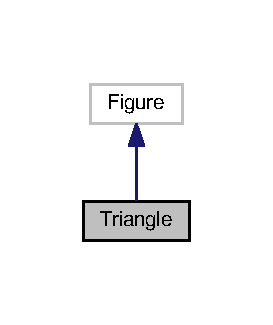
\includegraphics[width=131pt]{class_triangle__inherit__graph}
\end{center}
\end{figure}


Collaboration diagram for Triangle\+:
\nopagebreak
\begin{figure}[H]
\begin{center}
\leavevmode
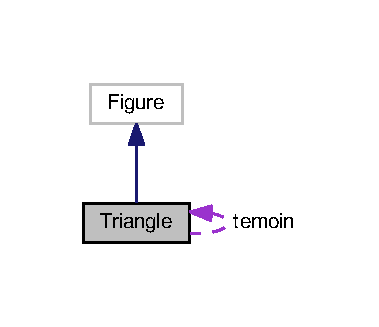
\includegraphics[width=182pt]{class_triangle__coll__graph}
\end{center}
\end{figure}
\subsection*{Public Member Functions}
\begin{DoxyCompactItemize}
\item 
{\bfseries Triangle} (const \hyperlink{class_point}{Point} \&a, const \hyperlink{class_point}{Point} \&b, const \hyperlink{class_point}{Point} \&c)\hypertarget{class_triangle_ad6736ceb2c5266d5654dc3e4dd6f5970}{}\label{class_triangle_ad6736ceb2c5266d5654dc3e4dd6f5970}

\item 
\hyperlink{class_point}{Point} {\bfseries getA} () const \hypertarget{class_triangle_a0dd6b0a5142764a033f8a2e4b9ced5c0}{}\label{class_triangle_a0dd6b0a5142764a033f8a2e4b9ced5c0}

\item 
\hyperlink{class_point}{Point} {\bfseries getB} () const \hypertarget{class_triangle_a1545c8812ce00318e49bd52e09d1e36a}{}\label{class_triangle_a1545c8812ce00318e49bd52e09d1e36a}

\item 
\hyperlink{class_point}{Point} {\bfseries getC} () const \hypertarget{class_triangle_a90c102c6b76c5feb2eaae27dd915dd4e}{}\label{class_triangle_a90c102c6b76c5feb2eaae27dd915dd4e}

\item 
virtual Figure $\ast$ \hyperlink{class_triangle_a42c97326207e09bf7d12f7a4b9fcd6d6}{copy} () const 
\item 
virtual list$<$ \hyperlink{class_point}{Point} $\ast$ $>$ {\bfseries get\+Points} () const \hypertarget{class_triangle_a301429604bdca0fb95b7b7bdda6184d6}{}\label{class_triangle_a301429604bdca0fb95b7b7bdda6184d6}

\item 
virtual void \hyperlink{class_triangle_ae44ae5995bcaba3cad9ca65a5ed14388}{deplacer} (const \hyperlink{class_point}{Point} \&trans)
\item 
virtual void \hyperlink{class_triangle_a7f91e70e78e8c296bae4f05c1788b051}{dessiner} (ostream \&os=cout) const 
\item 
virtual double \hyperlink{class_triangle_a621e89fd52c211202fa6109dcac3642e}{surface} () const 
\item 
virtual double {\bfseries perimetre} () const \hypertarget{class_triangle_a192e152f061780fee4b5680d689467aa}{}\label{class_triangle_a192e152f061780fee4b5680d689467aa}

\item 
virtual double {\bfseries distance\+\_\+origine} (const \hyperlink{class_point}{Point} \&p) const \hypertarget{class_triangle_a5d45ebaa6965729aa9956b28d5bf20d4}{}\label{class_triangle_a5d45ebaa6965729aa9956b28d5bf20d4}

\item 
virtual void {\bfseries afficher} (ostream \&os=cout) const \hypertarget{class_triangle_adb39ffbcfa9a0c1b8e24da01abc51bda}{}\label{class_triangle_adb39ffbcfa9a0c1b8e24da01abc51bda}

\end{DoxyCompactItemize}
\subsection*{Static Public Attributes}
\begin{DoxyCompactItemize}
\item 
static \hyperlink{class_triangle}{Triangle} \hyperlink{class_triangle_afdd6cbca626a9751730c23c18cf3967a}{temoin} = \hyperlink{class_triangle}{Triangle}(\hyperlink{class_point}{Point}(0,0), \hyperlink{class_point}{Point}(2,0), \hyperlink{class_point}{Point}(1,1))
\end{DoxyCompactItemize}


\subsection{Member Function Documentation}
\index{Triangle@{Triangle}!copy@{copy}}
\index{copy@{copy}!Triangle@{Triangle}}
\subsubsection[{\texorpdfstring{copy() const }{copy() const }}]{\setlength{\rightskip}{0pt plus 5cm}Figure $\ast$ Triangle\+::copy (
\begin{DoxyParamCaption}
{}
\end{DoxyParamCaption}
) const\hspace{0.3cm}{\ttfamily [virtual]}}\hypertarget{class_triangle_a42c97326207e09bf7d12f7a4b9fcd6d6}{}\label{class_triangle_a42c97326207e09bf7d12f7a4b9fcd6d6}
Fonction virtuelle de copie \index{Triangle@{Triangle}!deplacer@{deplacer}}
\index{deplacer@{deplacer}!Triangle@{Triangle}}
\subsubsection[{\texorpdfstring{deplacer(const Point \&trans)}{deplacer(const Point &trans)}}]{\setlength{\rightskip}{0pt plus 5cm}void Triangle\+::deplacer (
\begin{DoxyParamCaption}
\item[{const {\bf Point} \&}]{p}
\end{DoxyParamCaption}
)\hspace{0.3cm}{\ttfamily [virtual]}}\hypertarget{class_triangle_ae44ae5995bcaba3cad9ca65a5ed14388}{}\label{class_triangle_ae44ae5995bcaba3cad9ca65a5ed14388}
Déplacement-\/translation de valeur le point p \index{Triangle@{Triangle}!dessiner@{dessiner}}
\index{dessiner@{dessiner}!Triangle@{Triangle}}
\subsubsection[{\texorpdfstring{dessiner(ostream \&os=cout) const }{dessiner(ostream &os=cout) const }}]{\setlength{\rightskip}{0pt plus 5cm}void Triangle\+::dessiner (
\begin{DoxyParamCaption}
\item[{ostream \&}]{os = {\ttfamily cout}}
\end{DoxyParamCaption}
) const\hspace{0.3cm}{\ttfamily [virtual]}}\hypertarget{class_triangle_a7f91e70e78e8c296bae4f05c1788b051}{}\label{class_triangle_a7f91e70e78e8c296bae4f05c1788b051}
Le dessin se limite à un affichage \index{Triangle@{Triangle}!surface@{surface}}
\index{surface@{surface}!Triangle@{Triangle}}
\subsubsection[{\texorpdfstring{surface() const }{surface() const }}]{\setlength{\rightskip}{0pt plus 5cm}double Triangle\+::surface (
\begin{DoxyParamCaption}
{}
\end{DoxyParamCaption}
) const\hspace{0.3cm}{\ttfamily [virtual]}}\hypertarget{class_triangle_a621e89fd52c211202fa6109dcac3642e}{}\label{class_triangle_a621e89fd52c211202fa6109dcac3642e}
Calcul de la surface d\textquotesingle{}un triangle avec la formule d\textquotesingle{}Héron 

\subsection{Member Data Documentation}
\index{Triangle@{Triangle}!temoin@{temoin}}
\index{temoin@{temoin}!Triangle@{Triangle}}
\subsubsection[{\texorpdfstring{temoin}{temoin}}]{\setlength{\rightskip}{0pt plus 5cm}{\bf Triangle} Triangle\+::temoin = {\bf Triangle}({\bf Point}(0,0), {\bf Point}(2,0), {\bf Point}(1,1))\hspace{0.3cm}{\ttfamily [static]}}\hypertarget{class_triangle_afdd6cbca626a9751730c23c18cf3967a}{}\label{class_triangle_afdd6cbca626a9751730c23c18cf3967a}
Le triangle témoin est une variable de classe 

The documentation for this class was generated from the following files\+:\begin{DoxyCompactItemize}
\item 
archive/triangle.\+hpp\item 
archive/triangle.\+cpp\end{DoxyCompactItemize}

\chapter{File Documentation}
\hypertarget{_line_8cpp}{}\section{src/\+Line.cpp File Reference}
\label{_line_8cpp}\index{src/\+Line.\+cpp@{src/\+Line.\+cpp}}


Implementation d\textquotesingle{}une ligne.  


{\ttfamily \#include $<$cmath$>$}\\*
{\ttfamily \#include \char`\"{}Line.\+hpp\char`\"{}}\\*
Include dependency graph for Line.\+cpp\+:
\nopagebreak
\begin{figure}[H]
\begin{center}
\leavevmode
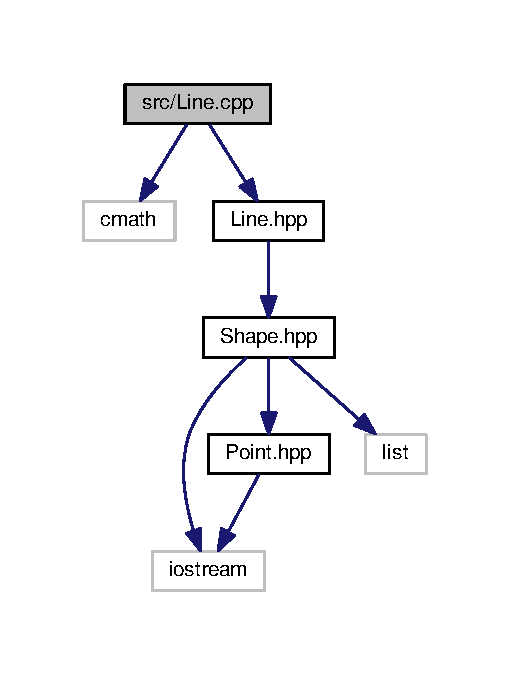
\includegraphics[width=245pt]{_line_8cpp__incl}
\end{center}
\end{figure}


\subsection{Detailed Description}
Implementation d\textquotesingle{}une ligne. 

\begin{DoxyAuthor}{Author}
M\+O\+R\+E\+A\+U.\+A Z\+E\+C\+C\+H\+I\+N\+I.\+A V\+I\+E\+R\+I\+A\+\_\+\+N\+O\+R\+O.\+K 
\end{DoxyAuthor}
\begin{DoxyVersion}{Version}
0.\+1 
\end{DoxyVersion}
\begin{DoxyDate}{Date}
13 mars 2018
\end{DoxyDate}
Impl�m�ntation d\textquotesingle{}une classe d�crivant une ligne dans une hi�rachie de figures. 
%--- End generated contents ---

% Index
\backmatter
\newpage
\phantomsection
\clearemptydoublepage
\addcontentsline{toc}{chapter}{Index}
\printindex

\end{document}
